\section{Semantic Consistency}

Our tools enforce a single view of the interpretation of design details in a design model.  
Consistency is required in both the structure of the design models (i.e. the componentization 
and its relations) as well as the behavior represented by the design models (i.e. the model of 
computation in which tasks are executed and their behavior within that model). 

\begin{figure}
\centering
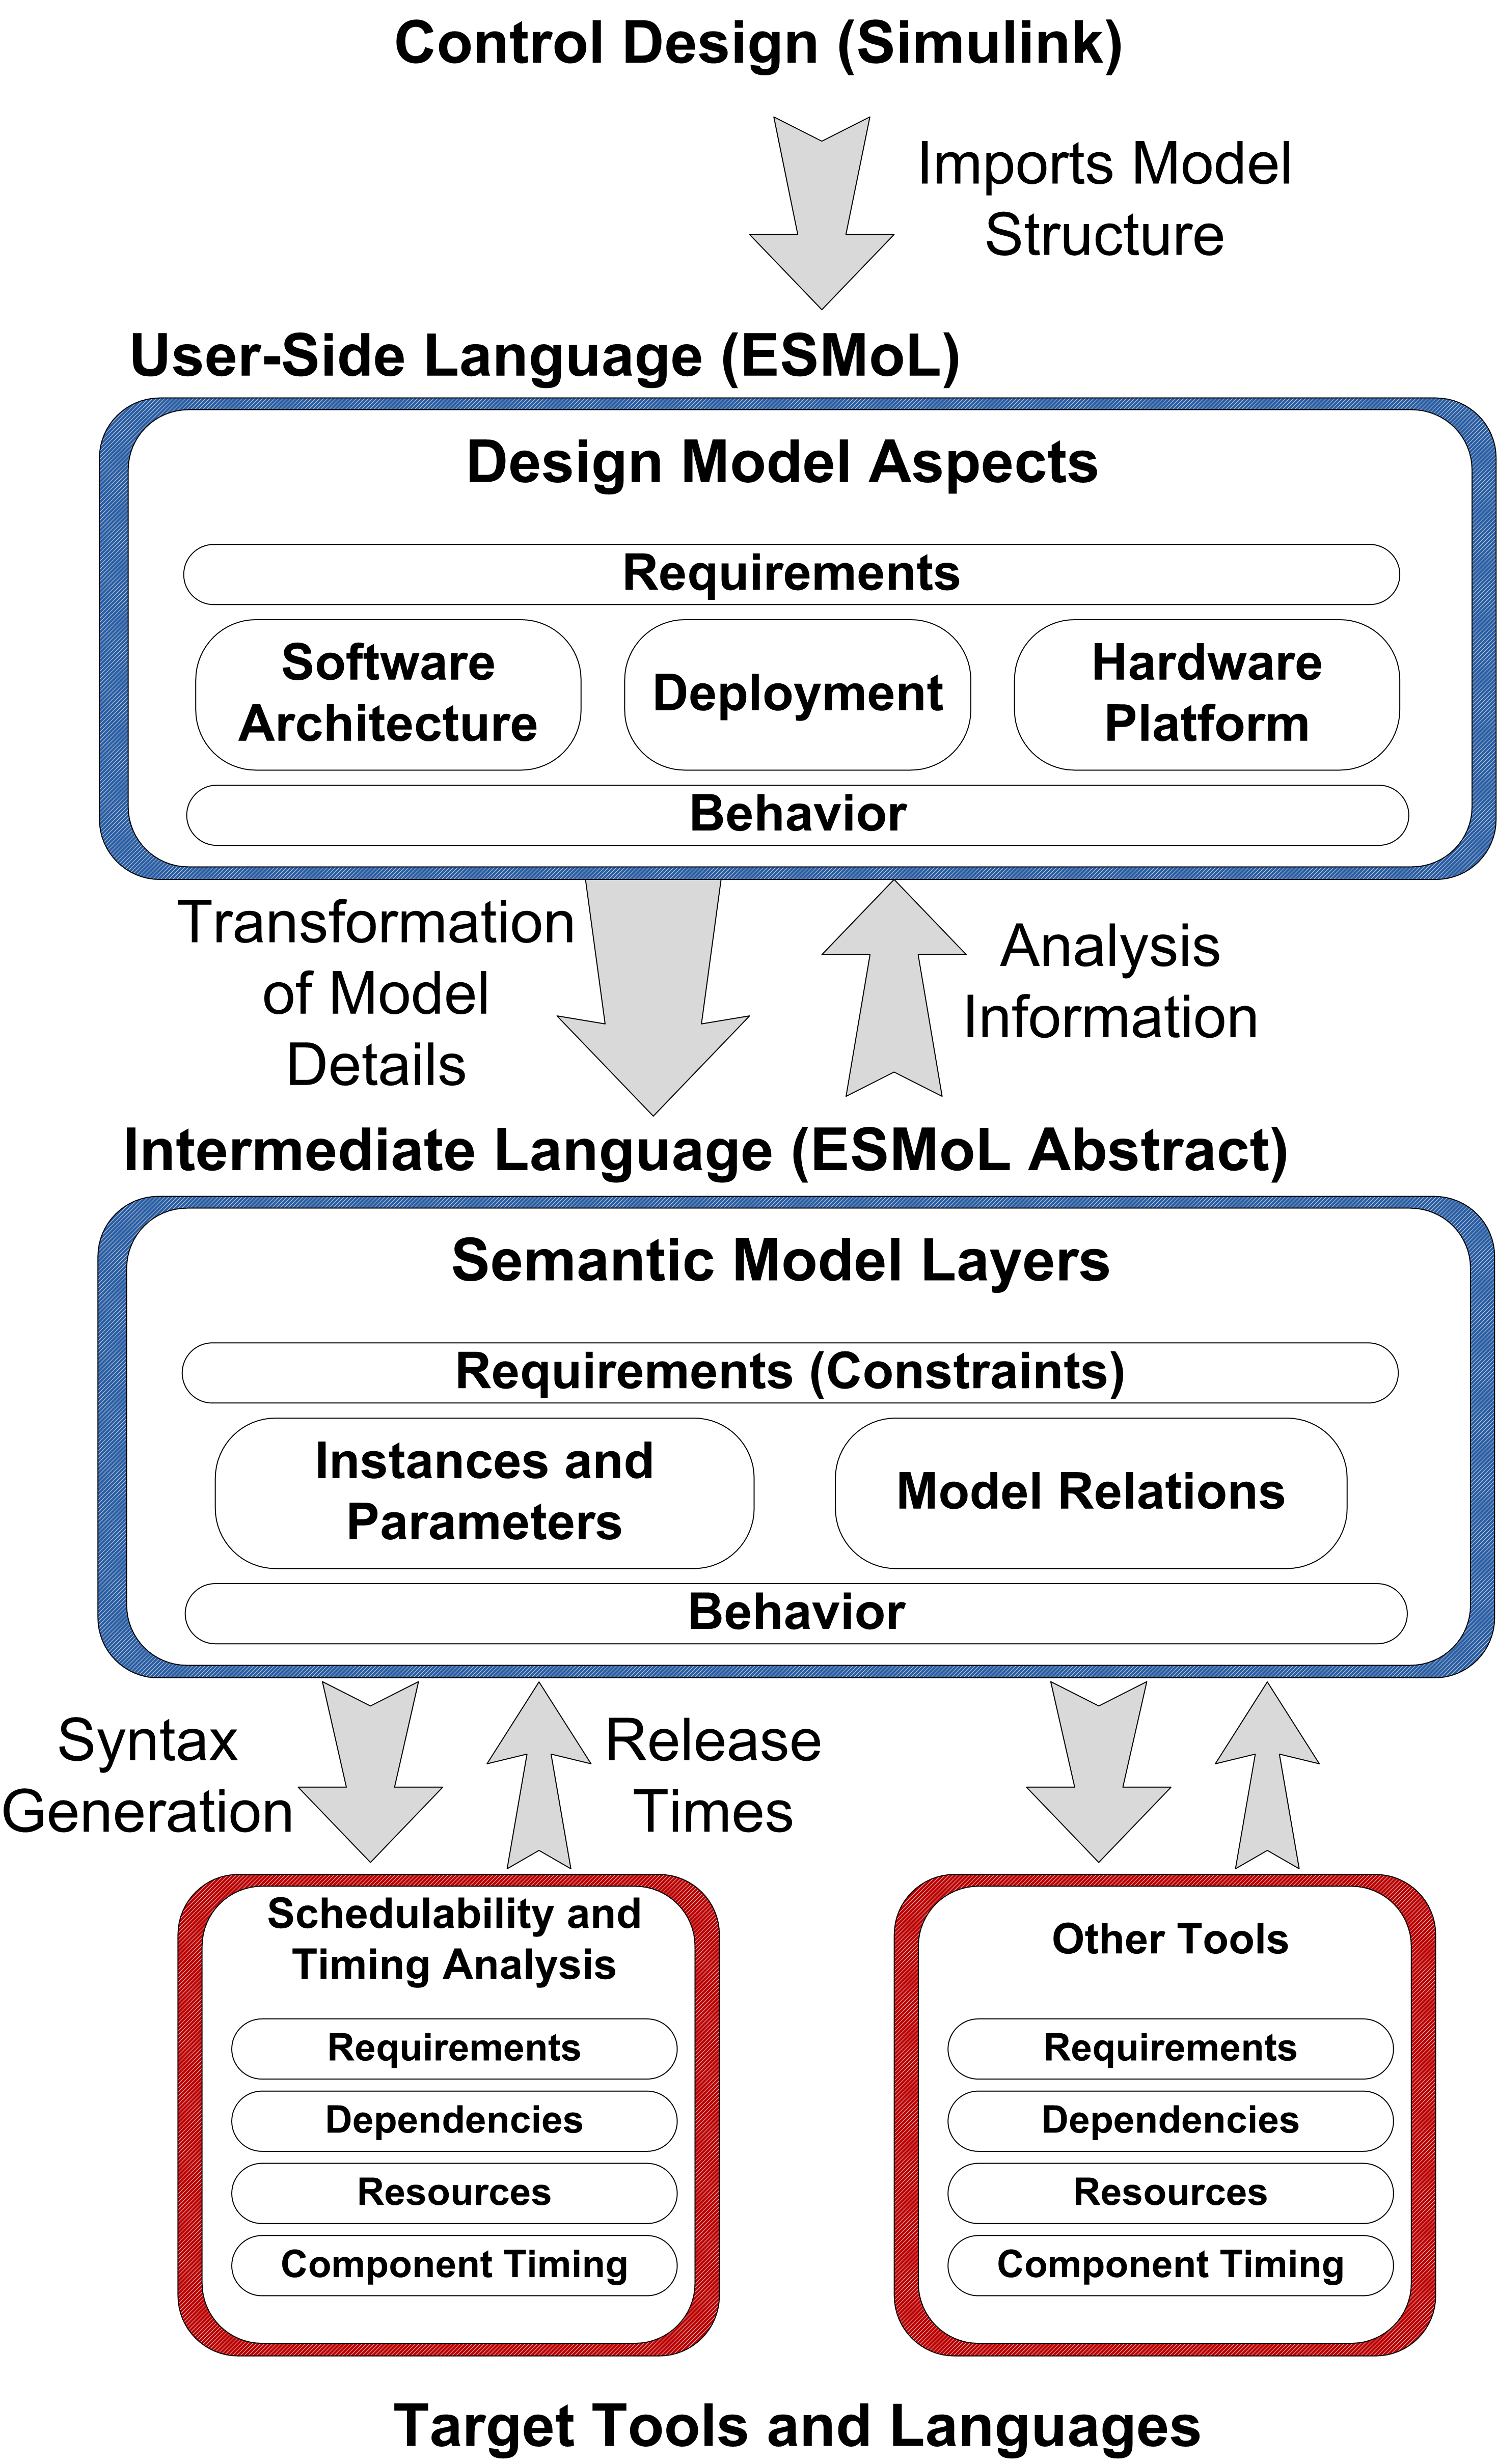
\includegraphics[width=0.72\columnwidth]{figures/designflow.png}
    \caption{Suggested flow of design models between design phases. During design iterations, 
analysis data can be transformed and fed back to designers. }
    \label{fig:designflow}
\end{figure}

The model-integrated computing approach (MIC) \cite{mic:overview} facilitates the essential 
part of the consistency effort.  Fig. \ref{fig:designflow} depicts a design flow that includes 
a user-facing modeling language for design and a language for explicit representation of semantics.  
In the Generic Modeling Environment (GME) \cite{mic:gme} a designer creates an embedded system 
software design from an imported Simulink control design.  Rather than designing a user-friendly 
graphical modeling language and directly attaching translators to analysis tools, we created a 
simple abstract intermediate language whose elements are similar to those of the user language. 
Mappings from the intermediate language to analysis tools are one-to-one (if possible), and 
semantically insignificant relationships (i.e. those used for visualization) are removed.  
The first model transformation flattens the user model into the intermediate form, resolving 
parameters and special cases as needed. New elements are only added to the intermediate language 
as required by the analysis tools.

The front end language, abstract intermediate language, and the transformation between them 
were designed and implemented together, in order to provide useful abstractions to the user 
and to the tool integrator.  Both languages are specified as layered metamodels 
\cite{mic:overview} which include elements for requirements, design structures, and behavioral 
models.   This translation is similar to the way a compiler translates concrete syntax first 
to an abstract syntax tree, and then to intermediate semantic representations suitable for optimization.

Each analysis translation works from a single view of the design model, keeping 
tool-specific translations simple.  As a simple example, consider Fig. \ref{fig:deps}, 
which comes from the user design model.   Component DataHandling sends data messages to 
the other two components, as denoted by the dependency arrows.  The behavioral semantics 
of this model are ambiguous at this point, as we have a dependencies but no timing 
specification.  The deployment view (Fig. \ref{fig:deploy} shows that each component 
executes on a different processor.  Locally, the port object on each component (in 
both diagrams) represents the component's view of the actual data message sent over the 
wire. The solid connections in the deployment diagram indicate which device on the processing 
node will be used to transfer the data.  Specified messages will participate in processor-local 
synchronous data flows, or time-triggered exchanges over the network.  All of these connections 
and entities are related to a single semantic message object, which is related to other elements 
in different parts of the user model (see the FormattedData message in Fig. \ref{fig:msg_sched}).  
We still have some ambiguity.  This is simply because different designers could make differing 
assumptions about the implementation of model details in their respective domains.  Numerous 
message handling implementations would work adequately for the specified design.  In the absence 
of other constraints (such as performance and efficiency), designers must choose implementation 
details.  The message transfer could consist of a single broadcast to $N$ receivers, or $N$ individual 
message transfers, so these cases must be specified unambiguously.

\begin{figure}
\centering
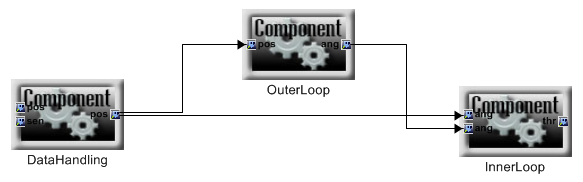
\includegraphics[width=0.9\columnwidth]{figures/dependencies.png}
    \caption{Three components (blocks) with message transfer dependencies (arrows). The dependency 
connection ports on each component represent the message instance as seen by the component.}
    \label{fig:deps}
\end{figure}


The first stage transformation checks constraints to ensure that each object is used 
consistently throughout the design, and then reduces this complex set of relations to 
a single message object with relations to the other objects that use it.  Timing parameters 
from the platform model are used to calculate a behavioral model for the message (provided 
by the scheduler, described below), including requested times to start transfers and duration 
of each message on the bus.

A more useful example of potential inconsistency appears in the interpretation of parameters.  
Assume that the designer of a code generator needs some way to flag a special case for generating 
task code, and so chooses a special interpretation of the task period parameter for the value 
zero.  If the tools integrate schedulability analysis (and the scheduler is unaware of the 
special case, as often happens) then we have a condition that may introduce a subtle error 
into the design via a false positive result.  In the two-stage framework, the interpretation 
of the special case would be represented in one place only.  Its result would be to generate 
a different set of objects, relations, and/or parameters in the intermediate language, reducing 
opportunities for different interpreter writers to make inconsistent assumptions about message 
objects implementation.

\begin{figure}
\centering
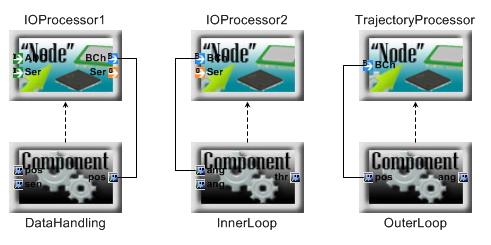
\includegraphics[width=0.9\columnwidth]{figures/deployment.png}
    \caption{Deployment model for the three components in the example.  Dashed arrows 
represent assignment of components to their respective processor, and solid lines represent 
assignment of message instances (component ports) to communication channels (port objects) 
on the processor.}
    \label{fig:deploy}
\end{figure}


The following sections (III, IV, and V) cover different aspects of a conceptual development 
process. We discuss semantics represented by the models, as well as information that could 
be provided back to the designers for further design iterations (see Fig. \ref{fig:designflow}).  
We also discuss details of some of the intermediate language structures relevant to each design 
stage.  While we do not have space to describe the full structural and behavioral semantics of 
the language, Table \ref{tab:consistencyTools} gives a brief summary of our current correctness 
arguments within the full semantics.  The front-end language, the intermediate language, and 
the first stage transformation work together to represent these assumptions and guarantees 
consistently.

\begin{table}
	\centering
		\begin{tabular}[width=0.75\columnwidth]{@{\extracolsep{\fill}} | p{1.2cm} | p{3.25cm} | p{3.05cm} | }
		\hline
		\multicolumn{3}{|c|}{Behavioral Consistency Concepts} \\
		\hline
		. & Execution Order Constraints & Timing Constraints \\ \hline \hline
		Dynamic Stability (Comp) & Passive controllers execute synchronously at a fixed rate determined by control analysis and simulation. & Control functions execute in bounded time, measured for the given platform. Nominal sample rates are passive and stable. \\ \hline
		Dynamic Stability (Intr) & Passive control design decreases the effects of delays from scheduling and platform timing jitter. Below we propose one abstraction for these effects. & Timing guarantees are not yet considered in our passive control design framework. \\ \hline
		\hline
	    Scheduling (Comp) & We use a synchronous data flow execution model to precompute component invocation order within tasks to eliminate local data hazards. & Each task has a known, bounded execution time (WCET/Deadline parameters are in the model).  \\ \hline
		Scheduling (Intr) & Message and task dependencies are translated to linear constraints, along with constraints to model resource utilization. & Scheduling achieves the desired sample rate and enforces latency bounds between tasks.  A proposed delay abstraction could represent schedule slack, and latency could be used to budget slack. \\ \hline
 \hline
		Execution Environment (Comp) & Statically precomputed task release times are used to configure the generated tasks, and the VM enforces start times. & We assume bounded-time task execution.  VM tasks can not be preempted, and so execute as quickly as possible to meet their deadline ( = WCET in this case). \\ \hline
		Execution Environment (Intr) & Clocks on separate nodes are synchronized to support synchronous execution.  Frame sync (null) messages are sent at the start of the common hyperperiod to keep nodes executing together.  & Time-triggered schedules prevent collisions, so messages transfer deterministically. Measured transfer overhead is captured in the platform design, and used in scheduling calculations. \\ \hline
		\end{tabular}
	\caption{Summary discussion of the behavioral consistency concerns from the point of view of each design stage of our tools so far.  The (Comp) notation refers to component (task) level concerns, and (Intr) refers to global interaction concerns.}
	\label{tab:consistencyTools}
\end{table}
